\chapter{Forest for the Trees}
\lettrine[lines=4]{T}{rees} are another special kind of graph which we did not discuss in the previous chapter. Trees are somewhat unique compared to the other types of specialty graphs described before as they allow us certain algorithms to perform to solve different problems. Before we go in depth into trees, we must first define an operation and some other terms.

\section{Definitions}
Let $G_1$ and $G_2$ be graphs. Then $G_1 \cup G_2$ is the \textbf{union} of $G_1$ and $G_2$ with the vertex set $V = V(G_1) \cup V(G_2)$ and edge set $E = E(G_1) \cup E(G_2)$. Now, let's establish some more definitions:
\begin{description}
    \item[Disconnected:] A graph is \textbf{disconnected} if it is the union of two graphs. Here is an example of a disconnected graph:
    \begin{center}
        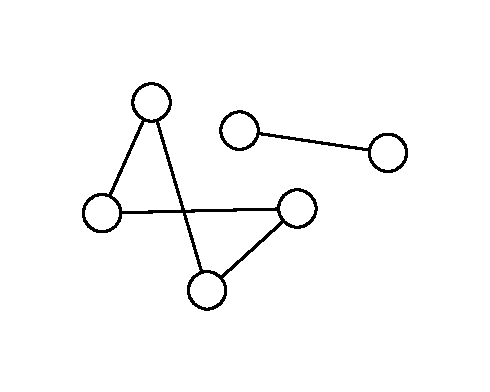
\includegraphics[width=0.3\textwidth]{Chapter2/disconnect.pdf}
    \end{center}
    \item[Connected:] A graph is \textbf{connected} if it is not disconnected (wow). Here is an example of a connected graph:
    \begin{center}
        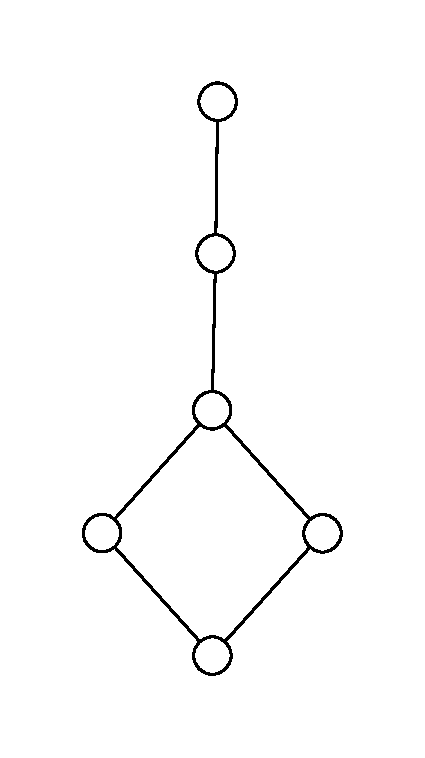
\includegraphics[width=0.3\textwidth]{Chapter2/connect.pdf}
    \end{center}
    \item[Component:] A \textbf{component} graph is one graph which makes up part of a union. In $G = G_1 \cup G_2$, $G_1$ and $G_2$ are components.
\end{description}

We can also define the \textbf{subtraction} of a set of edges $F$ from a graph $G$. We say that $G - F$ is the graph resulting in the removal of the edges in $F$ from $G$. Suppose we have the following graph $G$:
\begin{center}
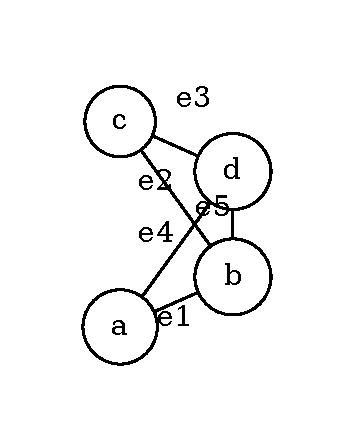
\includegraphics[width=0.3\textwidth]{Chapter2/sub0.pdf}
\end{center}
Then the following are different subtractions from $G$.
\begin{figure}[h]
    \subfloat[$G - \{e1\}$]{
        \begin{minipage}[c][1\width]{0.3\textwidth}
            \centering
            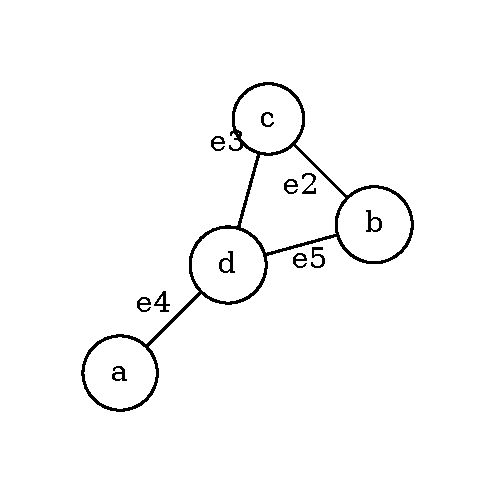
\includegraphics[width=1.\textwidth]{Chapter2/sub1.pdf}
        \end{minipage}
    }
    \subfloat[$G - \{e2\}$]{
        \begin{minipage}[c][1\width]{0.3\textwidth}
            \centering
            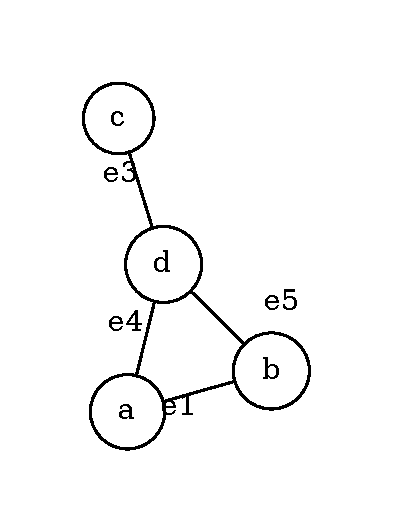
\includegraphics[width=\textwidth]{Chapter2/sub2.pdf}
        \end{minipage}
    }
    \subfloat[$G - \{e1, e2\}$]{
        \begin{minipage}[c][1\width]{0.3\textwidth}
            \centering
            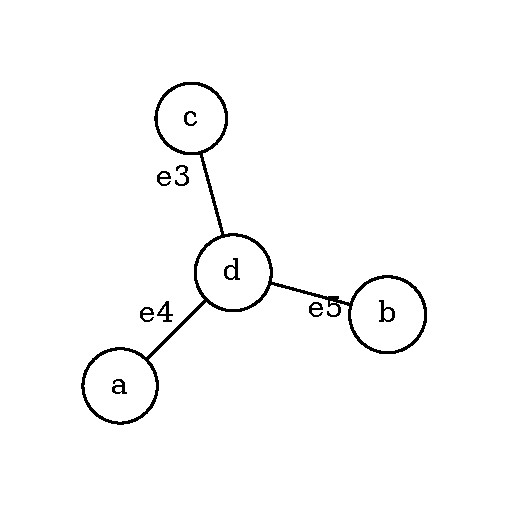
\includegraphics[width=\textwidth]{Chapter2/sub12.pdf}
        \end{minipage}
    }
\end{figure} 

Let's define a new type of graph. A connected graph that is regular of degree 2 is called a \textbf{cycle}, which we denote $C_n$. Here is an example of a cycle, $C_5$:
\begin{center}
    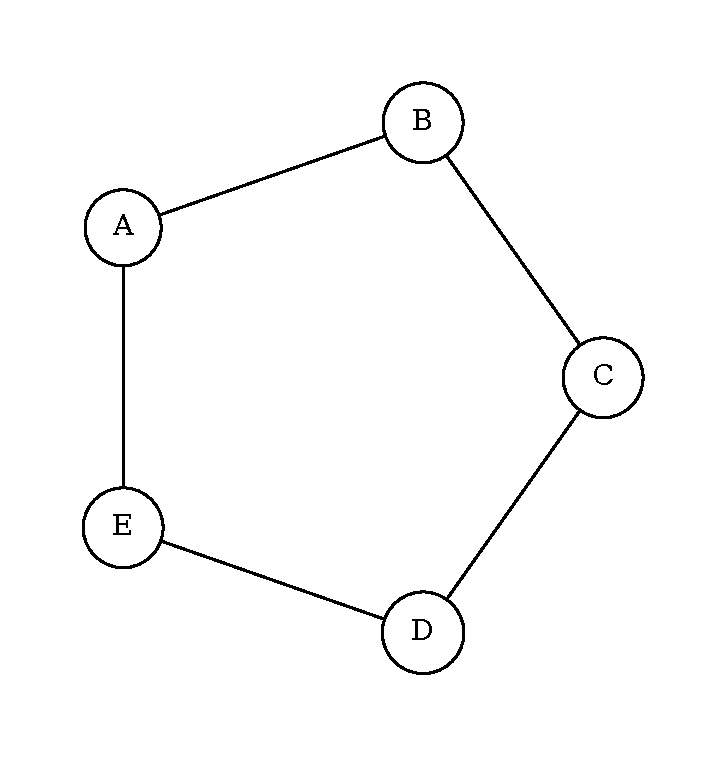
\includegraphics[width=0.3\textwidth]{Chapter2/c5.pdf}
\end{center}

A useful operation on graphs is to take the complement. The \textbf{complement} of a graph $G$ is the graph $\overline{G}$, with vertex set $V(\overline{G}) = V(G)$, with two vertices adjacent in $\overline{G}$ if and only if they are \emph{not} adjacent in $G$. Given $C_5$, we can fine its complement, $\overline{C_5}$:
\begin{center}
    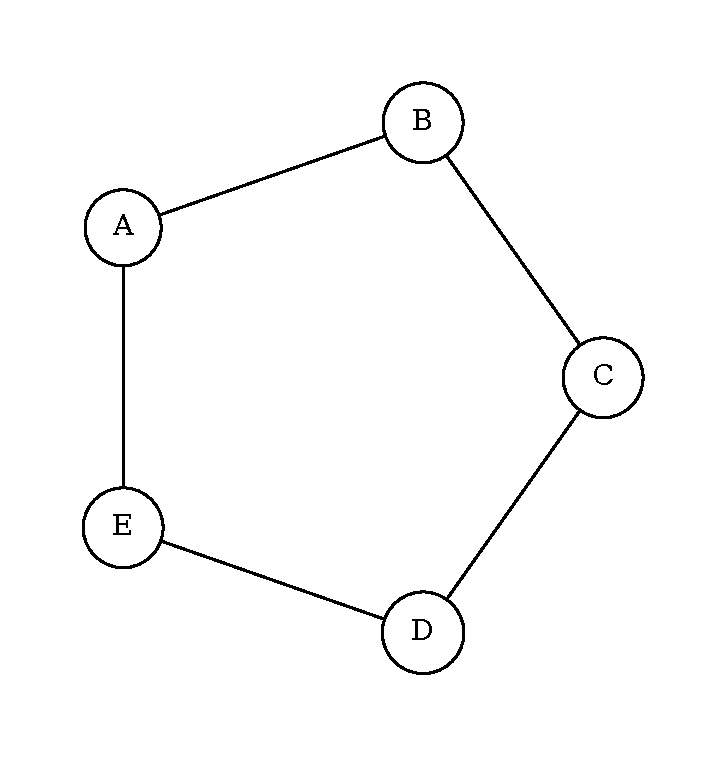
\includegraphics[width=0.3\textwidth]{Chapter2/c5.pdf}
    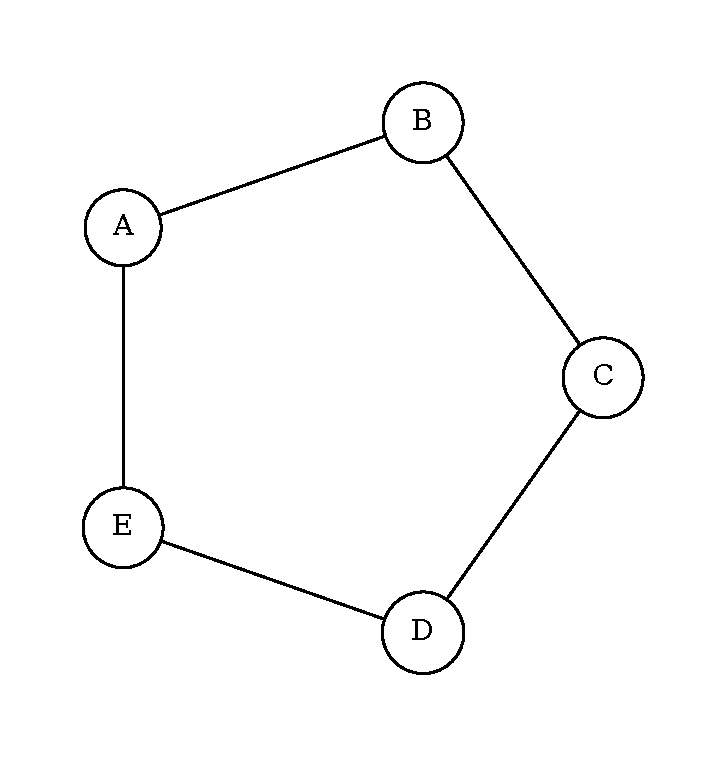
\includegraphics[width=0.3\textwidth]{Chapter2/c5.pdf}
\end{center}

\section{Trailblazing}
We've defined what graphs are as a construct, but how do we actually navigate from one point to another? There are different ways to navigate from vertex to vertex, as well as different forms of these navigations.